\documentclass{article}
\usepackage[utf8]{inputenc}
\usepackage{natbib}
\usepackage{graphicx}
\usepackage{textcomp}
\usepackage{amsmath}
\usepackage[T1]{fontenc}
\usepackage{graphicx}
\graphicspath{ {images/} }
\usepackage{amssymb}

\title{Assignment 2}
\author{Pratik Gaikwad}



\begin{document}

\maketitle

\section{Computational security}
    
    Consider a symmetric-key encryption
    \begin{center}
        $ \prod $ = (Gen, Enc, Dec)
    \end{center}
    
    \paragraph{Question 1:} What is a \emph{negligible function}, what is a \emph{PPT adversary}, and what is their importance in defining the computational security of 
    \begin{math} 
        \prod 
    \end{math} as a \emph{relaxation} of perfect secrecy?
    
    \paragraph{Answer:\newline} 
    
        \begin{flushleft}
            A function \emph{f} is called \emph{negligible function} \emph{if for every polynomial p(.) there exists an N such that for all integers n \textgreater N it holds that}
            \begin{center}
                $
                    f(n) = \frac{1}{p(n)}
                $
            \end{center}
            
            An algorithm \emph{A} is said to run in polynomial time if there exists a polynomial \emph{p(.)} such that, for every input 
                $
                    x\in\{0,1\}^*
                $.
            Such an algorithm is called Probabilistic polynomial time(PPT) algorithm.
            An adversary who can find the solution of \emph{A(x)} using PPT algorithm within at most \emph{p(|x|)} steps, where |x| denotes the length of string x, is called PPT adversary. \newline
            
            Computational security introduces two relaxations of the notion of perfect security:
            \begin{enumerate}
                \item Security is guaranteed only against  efficient (i.e. polynomial-time) adversaries;
                \item Negligible probability of success is allowed.
            \end{enumerate}
            Both of these relaxations are essential for achieving practical cryptographic schemes. i.e. they support the definition of computational secrecy in the sense that any computationally secure scheme can't be broken with practical computational power within reasonable time.
        \end{flushleft}
    
    \paragraph{Question 2:} How is $\prod$'s \emph{security parameter} typically related to the input and output of algorithm Gen?
    
    \paragraph{Answer: \newline}
        The security parameter $1^n$ is a representation of how strong output of key generation algorithm should be. The algorithm Gen's running time is a polynomial in the length of the input to the algorithm. The cryptographic operations have a running time that is asymptotically polynomial in the length of inputs and it follows that algorithms running time is asymptotically polynomial in the security parameter as the length of the inputs is the same as the security parameter. \newline
        Any key \emph{k} which is output of Gen($1^n$) satisfies $|k|\geq n$. Because now the length of output key \emph{k} defined by security parameter \emph{n}, it would make harder for an adversary to decipher or gain knowledge of plain text based on length of the cipher text as all the output would be of same length.
    
    \paragraph{Question 3:} Show that if \emph{$v_1$} is negligible function, then for any positive polynomial \emph{p}, the function \emph{$v_2$(n) = p(n).$v_1$(n)} is also negligible. What does this imply for an attacker that attempts to break $\prod$ by \emph{guessing} its n-bit key \emph{k}(which selected by Gen uniformly from all possible keys)?
    
    \paragraph{Answer: \newline}
        Consider any random polynomial positive q(n). Then p(n)q(n) is another polynomial. It is given that \emph{$v_1$} is negligible. As per our definition of negligible function,
        \begin{center}
            \begin{math}
                (\exists n_0)(\forall nn_0)(v_1\leq \frac{1}{p(n)q(n)})            
            \end{math}
        \end{center}
        Hence for all n \textgreater\ $n_0$,
        \begin{center}
            \begin{math}
                v_2 = p(n).v_1 \leq\ \frac{p(n)}{p(n)q(n)}\ = \frac{1}{q(n)}
            \end{math}
        \end{center}
        Thus for any random positive q(n), we have n $\in$ N such that for all n $\geq\ n_0$ is negligible $v_2 \leq\ \frac{1}{q(n)}$ which proves that $v_2$ is also negligible.
    \citep{section1question3}
    
    \paragraph{Question 4:} Is \emph{f(n)} negligible, and why if 
        \begin{enumerate}
            \item 
                \begin{math}
                    f(n) = \frac{{n^{10}}^5}{{2^n}^\frac{1}{2}}
                \end{math}
            \item
                \begin{math}
                    f(n) = \frac{{n^{-5}}^{10}}{{10^5}.{{n^{10}}^5}}
                \end{math}
        \end{enumerate}
        
    \paragraph{Answer: \newline}
        \begin{enumerate}
            \item 
                \begin{math}
                    f(n) = \frac{{n^{10}}^5}{{2^n}^\frac{1}{2}}\\
                    f(n) = {{n^{10}}^5}{{2^{-n}}^{\frac{1}{2}}}\\                    
                \end{math}
                where ${{2^{-n}}^{\frac{1}{2}}}$ represents a \emph{negligible} polynomial.
                Based on the closure properties \emph{poly * negligible = negligible} this function \emph{f(n)} is negligible.
            \item 
                \begin{math}
                    f(n) = \frac{{n^{-5}}^{10}}{{10^5}.{{n^{10}}^5}}\\
                    f(n) = \frac{{n^{-50}}.{n^{-50}}}{{10^5}}\\
                    f(n) = \frac{{n^{-100}}}{{10^5}}\\
                \end{math}
                In this case, none of the polynomials are negligible since for any positive value of n polynomial are not reducing to 0, hence in this case \emph{f(n)} is not negligible.
        \end{enumerate}
    
\section{EAV-Security}
    Recall the basic game-based definition for secrecy, EAV-security, and its alternative formulation, depicted in Figures 1 and 2, respectively. In both cases, a PPT adversary $\mathit{A}$ selects two messages in $\mathit{M}$, one of which is encrypted to form the challenge cipher-text $c_b$ that must be determined by $\mathit{A}$.
    
    \paragraph{Question 1:} Explain how the definition in Figure 1 intuitively captures the property that any efficient adversary $\mathit{A}$ \emph{can essentially only guess the challenge cipher-text}.
    
    \paragraph{Answer: \newline}
        Figure 1 indicates the attack of \emph{A} in the presence of an Adversary. The adversary is allowed to choose the messages $\mathit{m_0}$ and $\mathit{m_1}$. Thus, even though it knows that c is an encryption of one of these plain-text messages, it still cannot determine which one was encrypted. Hence we know that the probability of choosing correct $b\prime$ by $\mathit{A}$ is exactly $\frac{1}{2}$. The probability  This is similar to guessing the outcome of the game with or without calculation to any random experiment. And thus an adversary \emph{A} can only guess the challenge cipher-text. \cite{section2question12}
    
    \paragraph{Question 2:} Explain how the definition in Figure 2 intuitively captures the property that any efficient adversary $\mathit{A}$ \emph{behaves essentially the same no matter what the challenge cipher-text is}.
    \paragraph{Answer: \newline}
        Definition in Figure 2 states that an adversary $\mathit{A}$ cannot determine which plain-text was encrypted with probability significantly better than a random guess. An another way of formalizing the definition is to state that every adversary behaves the same way whether it sees an encryption of $\mathit{m_0}$ or $\mathit{m_1}$. Since A outputs a single bit, "behaving the same way" means that it outputs 1 with almost the same probability in each case. Here constant \emph{b} is used rather than being chosen at random. Hence definition essentially states that \emph{A} cannot determine whether it is running in experiment $PrivK-EAV2_{A,\prod'}$(n,0) or $PrivK-EAV2_{A,\prod'}$(n,1).
    
    \paragraph{Question 3:} Show that the alternative formulation of Figure 2 implies EAV-security as defined in Figure 1.
    \paragraph{Answer: \newline}
        In Figure 2, the only difference is that the bit \emph{b} is now constant in encryption scheme rather than choosing at random. 
        Even after this the probability of out of challenge cipher text by $\mathit{A}$ i.e. $b\prime$ is now increased by some negligible function \emph{v(n)}. But even with this increase in probability \emph{A} can't definitely say which message was encrypted with probability better than $\frac{1}{2}$ + \emph{v(n)}. Essentially Figure 2 implies security as defined in Figure 1.
    
    \paragraph{Question 4:} In reference to the game in Figure 1, how CPA-security and CCA-security extend EAV-security?
    \paragraph{Answer: \newline}
        CPA security is preserved since adversary \emph{A} is choosing the two messages to be encrypted but is unable to identify with probability more $\frac{1}{2}$ which one of two equal length message was encrypted using encryption scheme. This is even after he had made make polynomially many queries prior to sending the challenge messages to be encrypted by the encryption scheme. As the encryption is probabilistic and key generation is randomized, it would not be possible for an adversary to correctly guess the message from challenge cipher-text \newline \newline
        CCA security is preserved since based on challenge cipher-text bit $c_b$ adversary \emph{A} can't tell neither which message was encrypted nor it reveals about encryption scheme or any other relevant information, even though we gave selected message also to an adversary along with challenge cipher text bit $c_b$. Hence an adversary can't gain any useful knowledge of the scheme to predict future cipher text.

\section{On leaking, or hiding, the message length}
    Consider encryption scheme $\prod$ = (Gen, Enc, Dec) that is EAV-secure w.r.t. the definition in Figure 1.
    
    \paragraph{Question 1:} What does the condition $|m_0| = |m_1|$ capture? Does it weakens or strengthen $\prod$'s security?
    \paragraph{Answer: \newline}
        The limitation that $|m_0| = |m_1|$ imposes that length of selected messages should be same. As the key generated by \emph{Gen} will be of length of \emph{n}, the length of cipher text at the output of \emph{Enc} will be greater or equal to \emph{n}. \newline
        This will avoid leakage of any information about plain text from cipher text because of variance in length. Thus Indistinguishability of the encryption scheme increase which in turn strengthen $\prod$'s security.
        
    \paragraph{Question 2:} Let $PrivK-EAV2_{A,\prod'}$(n) be the game in Figure 1 where \emph{A} is allowed to choose challenge messages of \emph{arbitrary length} for breaking encryption scheme $\prod' = (Gen',Enc',Dec')$, and consider the security notion derived by this modified game: Intuitively, $\prod'$ is EAV2-secure, if no efficient \emph{A} can determine $c_b$ better than guessing, even when $|m_0| \neq |m_1|$. Show that no EAV2-secure scheme $\prod'$ exists.
    \paragraph{Answer: \newline}
        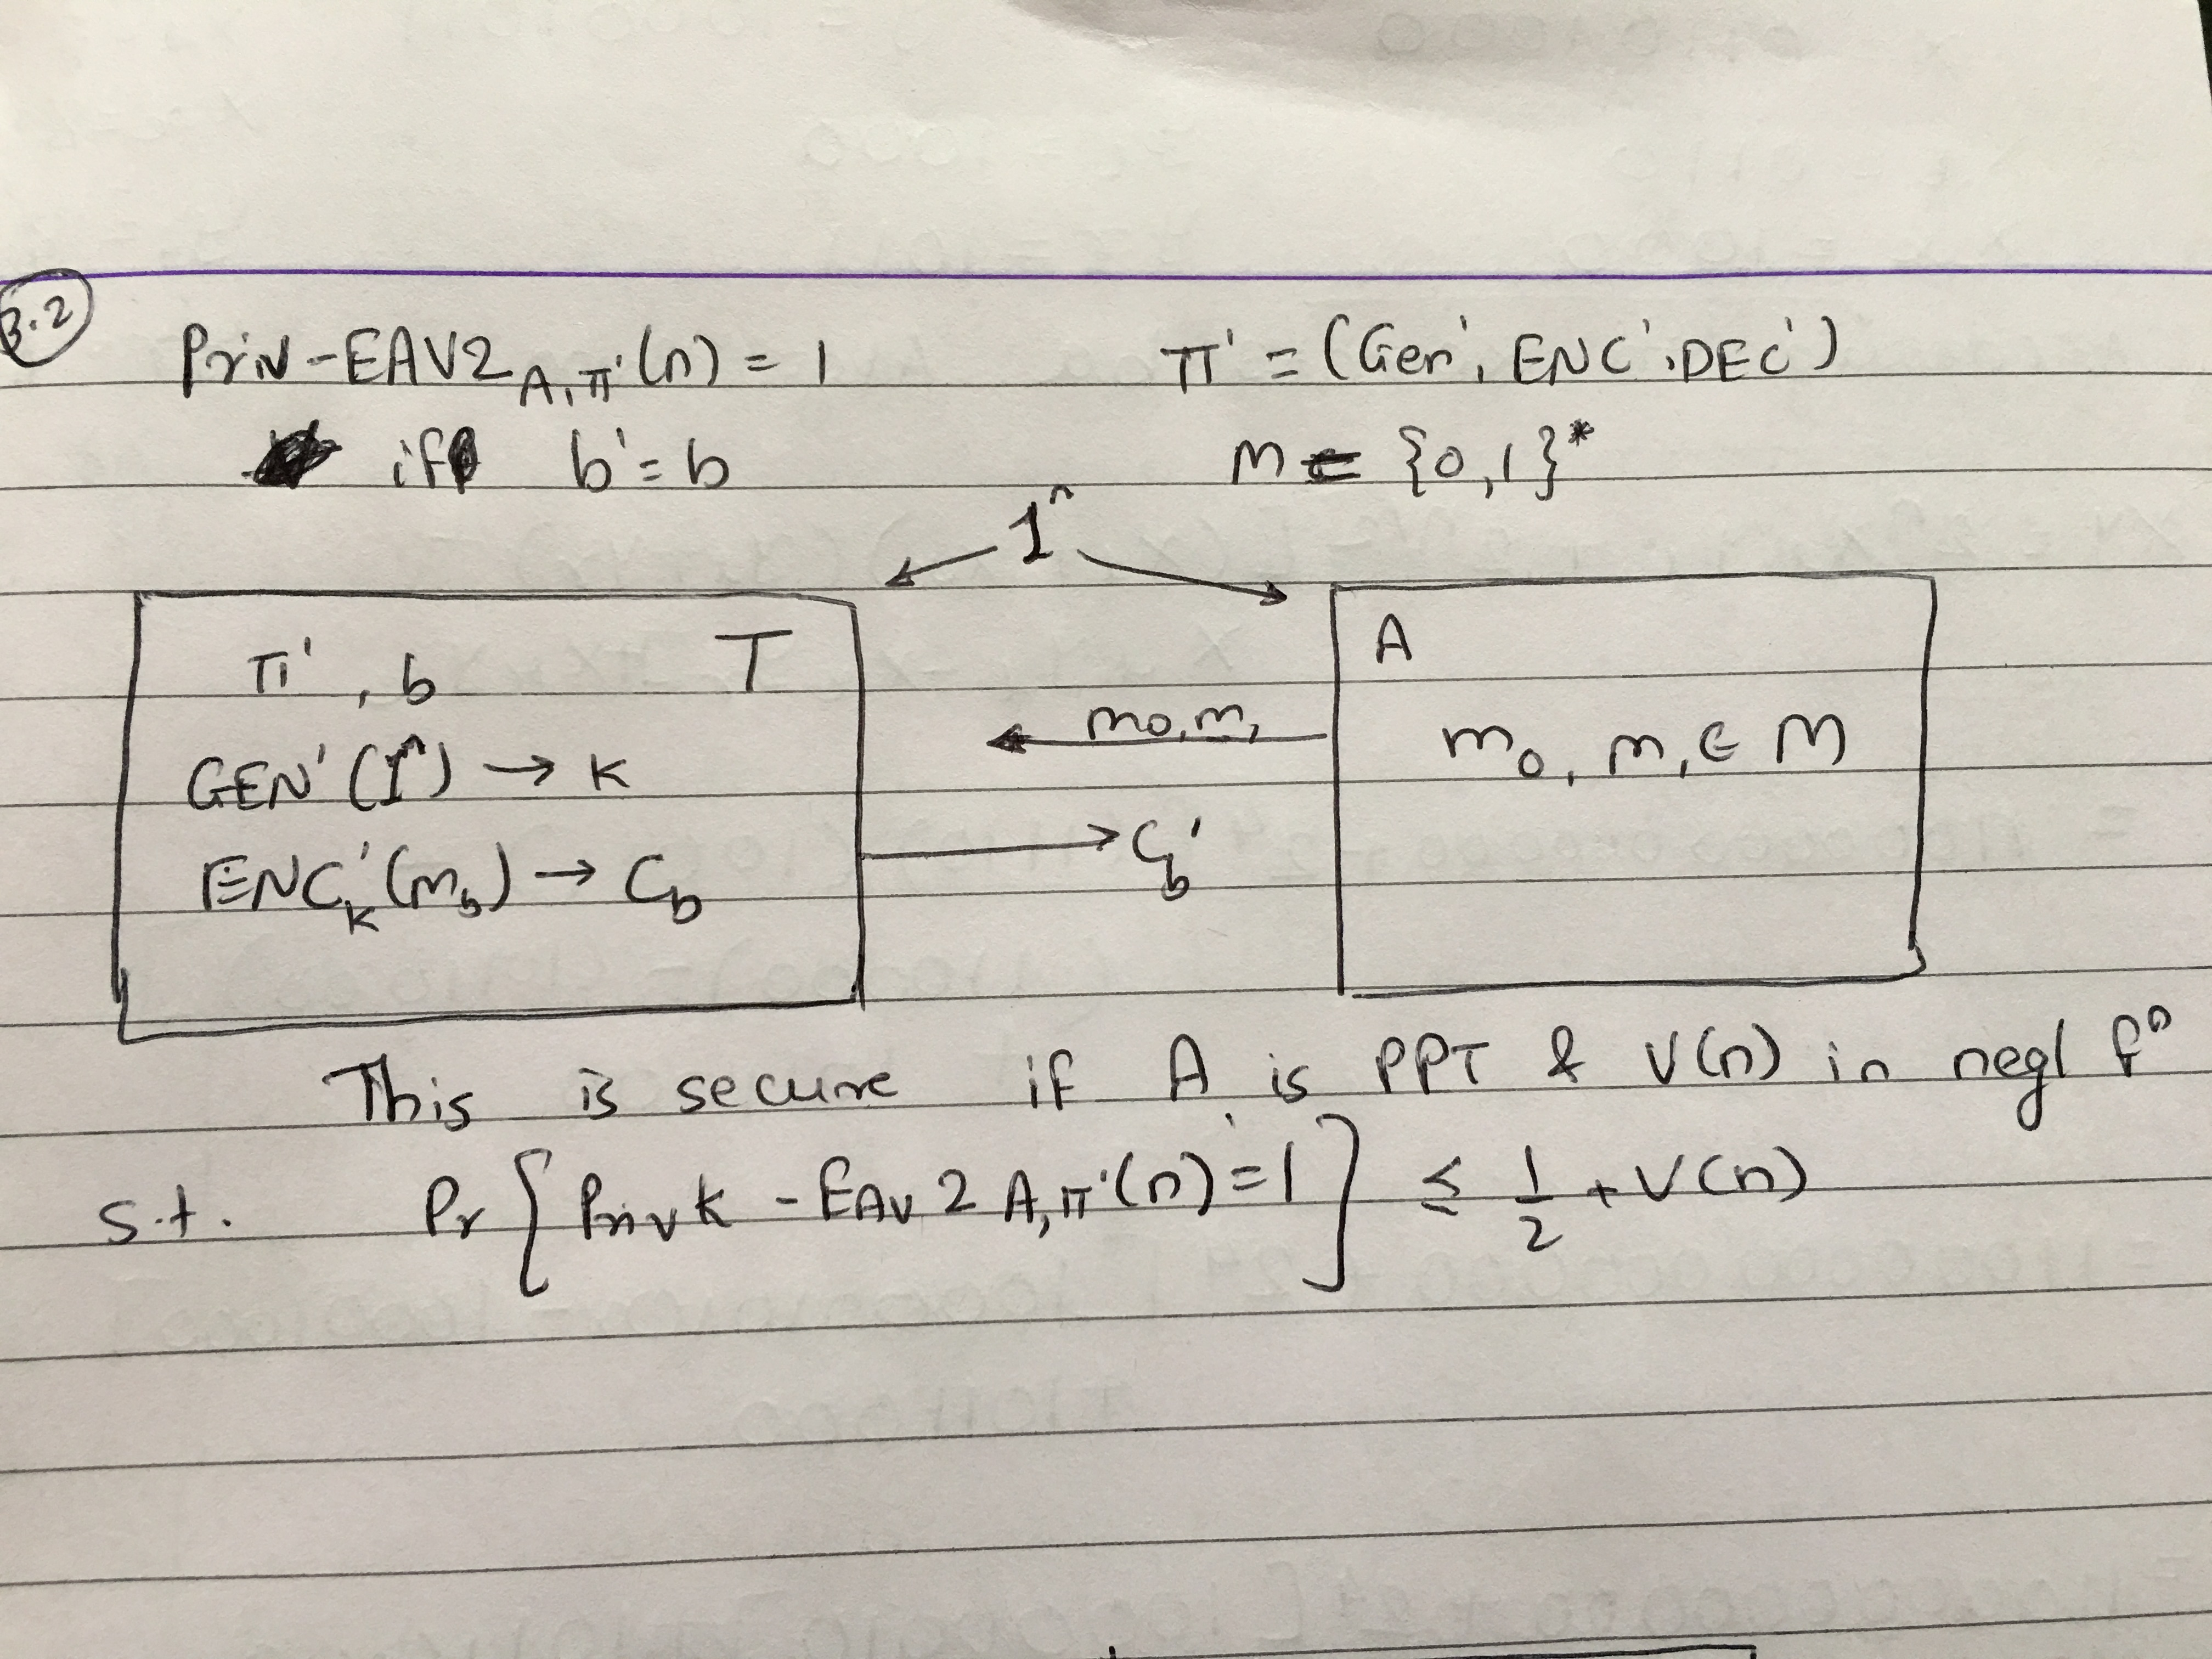
\includegraphics[scale=0.1]{S3Q2}
        \newline\newline
        Encryption scheme $\prod\prime$ will be as shown above. Let's consider that it takes maximum \emph{P(n)} to encrypt a single bit. As it is given that $|m_0| \neq |m_1|$, an adversary can choose \newline
        \begin{center}
            $m_0 \in {\{0,1\}}$ \\
            and $m_1 \in {\{0,1\}}^{P(n)+c}$\\
        \end{center}
        where c > 0. \\
        The length of output of $\prod\prime$ will be different and thus adversary can distinguish between two cipher-text messages with probability more than $\frac{1}{2}$. And hence this isn't secure scheme.
        
    \paragraph{Question 3:} Show that EAV2-security can be achieved by encryption schemes defined over messages up to  a given maximum length. i.e. by schemes $\prod\prime$ such that for $k \in {\{0,1\}}^n$, algorithm ${Enc\prime}_k$ is defined over message space ${M\prime}={\{m:|m|\leq l\}}$ where $l\triangleq l(n)$ for given polynomial $l(.)$
    
    \paragraph{Answer: \newline}
        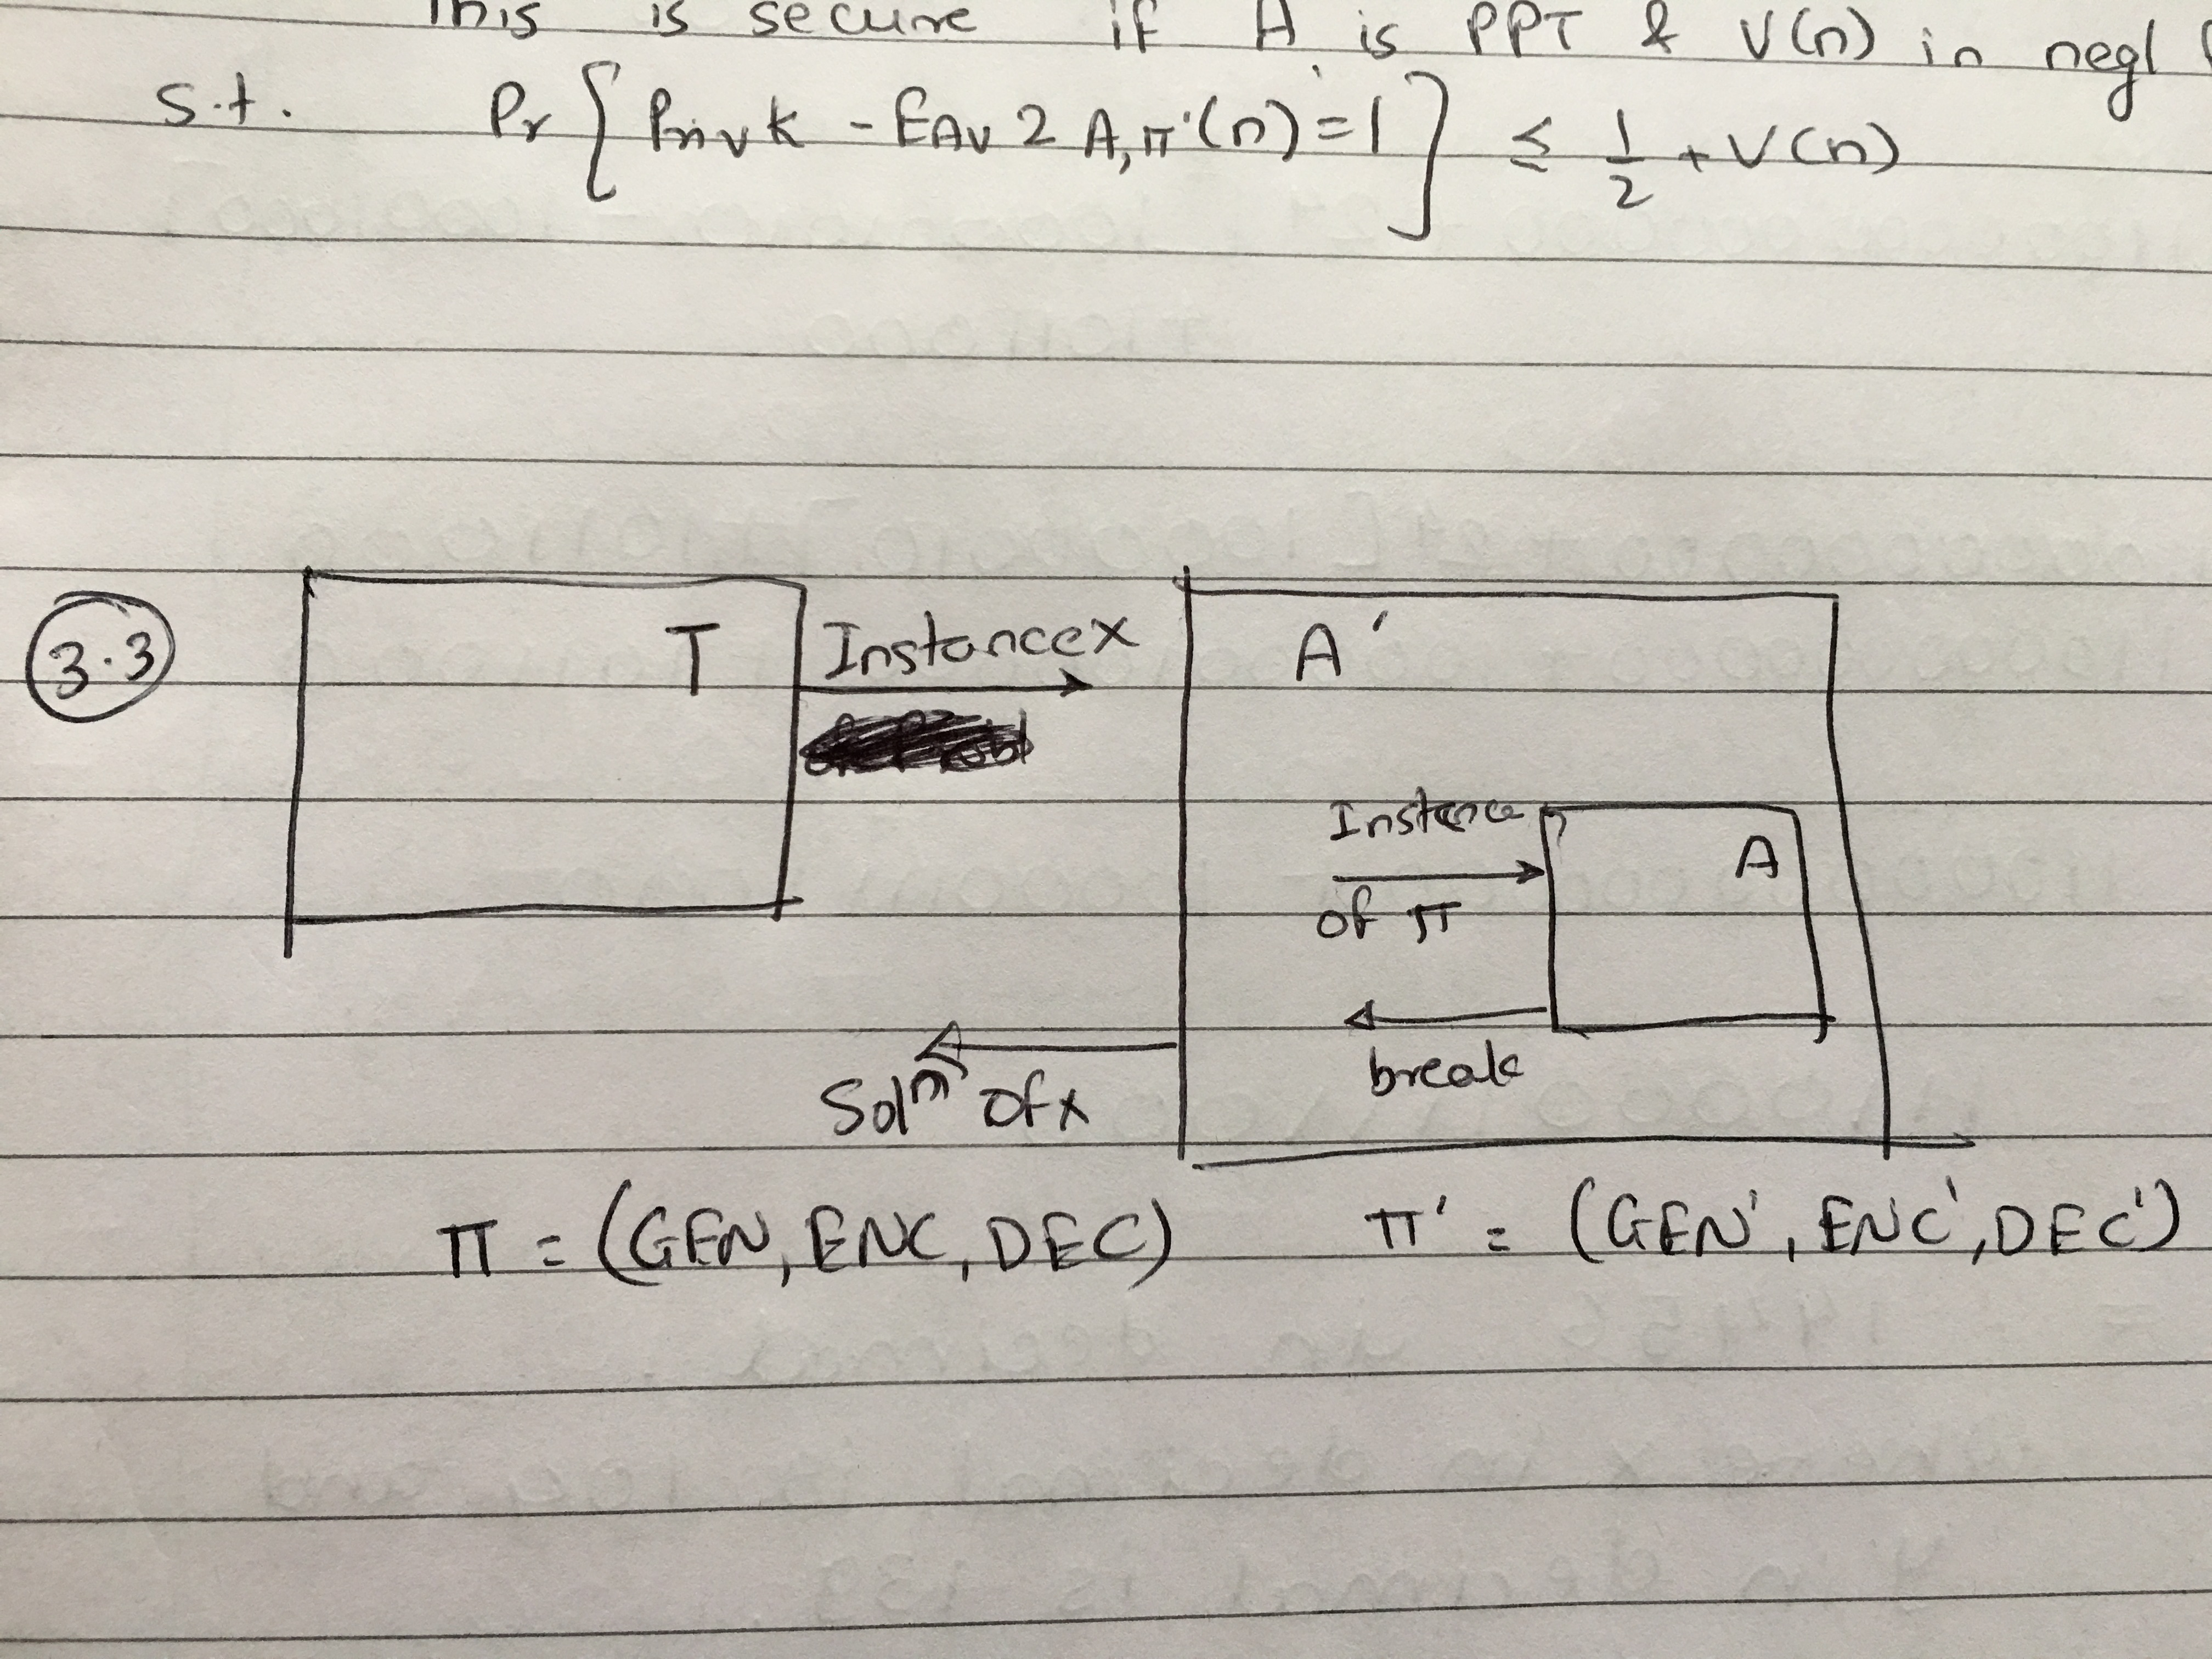
\includegraphics[scale=0.1]{S3Q3}
        \newline\newline
        Scheme \emph{A} is used as a subroutine for reduction in $A\prime$. In ${PrivK-EAV_{A,\prod}}: |m_0|=|m_1|$, however no such restriction is in ${PrivK-EAV_{A,\prod\prime}}$. It is given that ${\{m:|m|\leq l\}}$.
        The scheme $\prod\prime$ will be as follows:
        \begin{enumerate}
            \item $Gen\prime$ is similar to Gen.
            \item $Enc\prime$ receives message ${\{m:|m|\leq l\}}$ and creates cipher-text $c\prime \leftarrow{Enc_k{(m\prime)}}$
            \item $Dec\prime$ outputs message $m\prime:=Dec_k{(c\prime)}$
        \end{enumerate}
        With respect to above definition, let's assume that $\prod\prime$ is not secure. This assumption leads to assumption that $A\prime$ finds the solution in non-negligible probability in polynomial time.\newline
        Using \emph{A}, $A\prime$ solves \emph{T} with probability \emph{a(n)}. $A\prime$ gets the solution from \emph{A}. Since it is give that $\prod$ is secure then \emph{A} solves \emph{T} with negligible probability \emph{b(n)}. $A\prime$ after obtaining solution from \emph{A}, solves \emph{T} with probability \emph{c(n)}. \newline
        This indicates that,
        \begin{center}
            $Pr[A\prime = 1] = a(n).b(n).c(n)$
        \end{center}
        As $\prod$ is secure, \emph{b(n)} is negligible. and \emph{a(n),b(n)} = 1-(negligible term). if \emph{a(n).c(n)} has lower bound of $\frac{1}{p(n)}$ where p(n) is polynomial then,
        \begin{center}
            $Pr[A\prime=1] \geq \frac{b(n)}{p(n)}$\newline
        \end{center}
        This contradicts that $A\prime$ solves \emph{T} in polynomial time since negligible * negligible = negligible. And we can say that $A\prime$ is EAV2-secure.
        
    
\section{Pseudo-randomness \& modes of encryption}
    Recall the definitions of pseudo-random generators (PRGs) and pseudo-random functions (PRFs).
    
    \paragraph{Question 1:} If \emph{H}:$\{0,1\}^{l(n)}$ is a PRG with expansion factor \emph{l(n)} $\geq$ \emph{2n}, then G(H) = $H(s_1,s_2,..., s_{\frac{n}{2}})$, where s = $s_1,s_2,..., s_{\frac{n}{2}}$ is also a PRG. Determine whether $G\prime(s)=G(0^{|s|}||s)$ is necessarily a PRG, when \emph{G} is PRG.
    
    \paragraph{Answer: \newline}
        If a string of length \emph{2n} is given, then we can divide it in two n-bits string \emph{s||t}. The output of $G\prime$ is 1 if ${F_s}(0^n) = t$. This type of distinguishing is PPT. Also $Pr_{s\leftarrow{\{0,1\}^n}}[D(G(s)) = 1]$. If input = \emph{s||t} is random then the probability that \emph{t} is equal to $F_s{(0^n)}$ is exactly $2^{-n}$ and so $Pr_{s\leftarrow{\{0,1\}^n}}[D(s) = 1] = 2^{-n}$. This computation can be done with non-negligible probability ${1-2^{-n}}$. Hence $G\prime$ is not necessarily a PRG.
    
    \paragraph{Question 2:} If $F_k$ is a length-preserving PRF, determine whether the keyed function ${F\prime}_k:{\{0,1\}}^{n-1}\rightarrow{\{0,1\}}^{2n}$, with ${F\prime}_k=F_k(0||x)||F_k(x||1)$, is also a PRF.
    \paragraph{Answer: \newline}
        The pseudo-random function is defined as, $\forall$ PPT distinguisher D $\exists$ a negligible function s.t.
        \begin{center}
            $|Pr[D^{F_k(.)}(1^n) = 1] - Pr[D^{f(.)}(1^n) = 1] \leq negl(n)$
        \end{center}
        Let us consider \emph{D} a distinguisher with an \emph{Oracle} access to pseudo-random function $F\prime_k$ and randomly selected uniform function $f\prime$.
        In case of \emph{Oracle} access to pseudo-random function $F\prime_k$, \emph{D} queries with two inputs $x_1,x_2 s.t. x_1 \neq x_2$ with length (n-1). The distiguisher outputs 1 $\iff x_1||x_2 = y_1||y_2$. \newline
        Thus, $y_1||y_2 = F\prime_k(x_1)||F\prime_k(x_2) = F_k(0||x_1)||F_k(x_1||1)||F_k(0||x_2)||F_k(x_2||1) = x_1||x_2$.\newline
        In case of \emph{Oracle} access to random function $f\prime$, $Pr[y_1||y_2 = x_1||x_2] = \frac{1}{2^n}$\newline
        Thus the difference between these two probabilities is $\geq 1 - \frac{1}{2^n}$. This contradicts the definition of pseudo-random function as mentioned above. And hence $F\prime_k(x)$ is not PRF.
        
    \paragraph{Question 3:} If G is PRG with expansion factor $l(n)=n+1$ and \emph{F} is a PRF, determine whether each of the following encryption scheme with secret key a random $k \in {\{0,1\}}^n$, is EAV- and/or CPA- secure. 
    \begin{enumerate}
        \item Message $m \in {\{0,1\}}^n+1$ is encrypted as $r||G(r)\oplus{m}$ where r is chosen uniformly in ${\{0,1\}}^n$;
        \item Message $m \in {\{0,1\}}^n$ is encrypted as $m\oplus{F(0^n)}$.
    \end{enumerate}    
    \paragraph{Answer: \newline}
        \begin{enumerate}
            \item If we consider input as $r||G(r)\oplus{m}$ then \emph{m} can be computed within PPT from G(r) as $G(r)(\oplus{G(r) \oplus{m})} = m$.\newline
            Thus this scheme is neither EAV- nor CPA- secure.
            \item Since F is a PRF and encryption is deterministic this is EAV-secure but not CPA-secure. since message $Enc(m \in {\{0,1\}}^n) = m \oplus{F(0^n)}$
        \end{enumerate}
    
    \paragraph{Question 4:} When using the CBC, OFB and CTR modes of operation what is the effect of: a) a single-bit error in the cipher text and b) a dropped cipher-text block)?
    \paragraph{Answer: \newline}
        \begin{enumerate}
            \item CBC mode: In CBC mode, plain text message is XOR-ed with output of previous block before adding to encryption. An initial Vector(IV) is used for initial block. 
                \begin{enumerate}
                    \item A single bit error in cipher-text: \newline
                    In this case, the error will propagate through next cipher blocks since the output of one block is used as input to XOR function. Further, the position of erroneous bit will remain same in all the next cipher blocks. Since the error is propagated, the decrypted output will differ significantly from original plain-text message.
                    \item Dropped cipher-text block:\newline
                    In this case, the plain text of the dropped block will not be available. This will also break the decryption chain since there won't previous cipher-text block is used as an input to XOR for decryption to get the plain text. The output of all the next blocks will be affected and will be different than original plain text.
                \end{enumerate}
            \item OFB mode: In OFB mode, output of previous encryption block before being XOR-ed with plain-text is used as input to next block. An initial vector is used for first block.
                \begin{enumerate}
                    \item A single bit error in cipher-text:\newline
                    In this case, the error will not propagate to next block but it will remain in the same location and in the same block. The decrypted output won't differ much from original plain-text.
                    \item Dropped cipher-text block: \newline
                    In this case, similar to CBC, the plain text related to dropped block will not be available. But this will not affect next blocks since the cipher text is not used as input to next blocks and in this sense OFB is auto-recoverable.
                \end{enumerate}
            \item CTR mode: In CTR mode, there is no feedback. pseudo-randomness in the key stream is achieved using a counter. An \emph{n} bit counter is used to an initial predefined value and increased with predefined rule. Plain-text message are then XOR-ed with encrypted value of the counter.
                \begin{enumerate}
                    \item A single bit error in cipher-text:\newline
                        This will be similar to OFB mode. Since the output of one block is not fed to another, the error will not propagate. It will remain in the same location and in the same block. The decrypted output won't differ much from original plain-text.
                    \item Dropped cipher-text block: \newline
                    In this case, decryption of that block only will not be available. Since there is no feedback or chaining, other blocks will not be affected.            
                \end{enumerate}
        \end{enumerate}

\section{Problem 5: Message authentication codes}
    
    let $\prod = (Gen,Mac,Vrfy)$ be a MAC that is secure according to the security definition in Figure 3.
    
    \paragraph{Question 1:} Consider the notion of $MAC_v$-security, namely the extension of the basic MAC-security defined in Figure 3 that results by allowing the adversary \emph{A} in game Mac-forge$_{A,\prod}(n)$ to have access to the Vrfy(.). Prove that if (Mac-secure) $\prod$ is a \emph{deterministic} MAC using \emph{canonical} verification, then $\prod$ is also MAC$_v$-secure.
    
    \paragraph{Answer: \newline}
        We get unique but same tag \emph{t} for any query \emph{Q} on any message \emph{m}, this is because it is given that the MAC is \emph{deterministic}. \newline
         As \emph{A} has access to both \emph{Mac} and \emph{Vrfy}. \newline
        i.e.
        \begin{center}
            $A^{Mac_k(.)} = A^{Mac_k(.),Vrfy_k(.)}$
        \end{center}
        Thus since MAC-secure(as shown in Figure 3) is same as Mac$_s$-secure with canonical form, it guarantees Mac$_v$-secure.
    
    \paragraph{Question 2:} Let \emph{F} be a PRF, $\langle i \rangle$ denote an $\frac{n}{2}$ encoding of integer \emph{i} and \emph{k} a uniform key in ${\{0,1\}}^n$. Show that the following MACs defined over messages $m=(m_1,m_2), m_i \in {\{0,1\}}^{\frac{n}{2}}$, are insecure.
        \begin{enumerate}
            \item The tag message $m = m_1,m_2$ is $t={F_k}(\langle 1 \rangle || {m_1}) \oplus {F_k}(\langle 2 \rangle || {m_2})$
            \item The tag message $m = m_1,m_2$ is (\emph{r,t}), where $t={F_k}(r)\oplus {F_k}(\langle 1 \rangle || {m_1}) \oplus {F_k}(\langle 2 \rangle || {m_2})$
        \end{enumerate}
        
    \paragraph{Answer: \newline}
        \begin{enumerate}
            \item
                The tags for message $m=m_1,m_2$ is $t={F_k}(\langle 1 \rangle || {m_1}) \oplus {F_k}(\langle 2 \rangle || {m_2})$. From the security parameter $1^n$ lets assume that \emph{A} makes two queries such that $m_1 = 0^{\frac{n}{2}} and m_2 = 1^{\frac{n}{2}} = 1^\frac{n}{2}$
                \begin{math}                
                    t={F_k}(\langle 1 \rangle || {m_1}) \oplus {F_k}(\langle 2 \rangle || {m_2})\newline
                    t={F_k}(\langle 1 \rangle || 0^\frac{n}{2}) \oplus {F_k}(\langle 2 \rangle || 1^\frac{n}{2})\newline
                    t=MAC_k(0^\frac{n}{2},1^\frac{n}{2})
                \end{math}
                Thus \emph{A} with probability 1 and MAC is not secure.
                
            \item
                The tag message $m = m_1,m_2$ is (\emph{r,t}), where $t={F_k}(r)\oplus {F_k}(\langle 1 \rangle || {m_1}) \oplus {F_k}(\langle 2 \rangle || {m_2})$
                Let's assume $m_i$ chosen uniformly at random such that $r=\langle1\rangle||m_i$\newline
                $t=F_k(r)\oplus{F_k(\langle1\rangle||m_i)}$\newline
                $t=F_k(r)\oplus{F_k(r)}$\newline
                $t=0^n$
                Thus this scheme doesn't request any tag. Since for the above case tag generated would be $\langle r, 0^n\rangle$ is valid tag for $m_1$. This indicates that \emph{A} wins with probability 1 and MAC is not secure.
        \end{enumerate}
    
    \paragraph{Question 3:} Consider the modification of basic CBC-MAC, where a random initial block is used each time a message is authenticated. Namely, to authenticate message $m_1,...,m_l$ choose uniform $t_0 \leftarrow{{\{0,1\}}^n}$, run a basic CBC-MAC over augmented message $t_0,m_1,...,m_l$ to get tag $t_l$, and output tag $\langle{t_0,t_1}\rangle$. Show that this modification yields an insure MAC.
    \paragraph{Answer: \newline}
        Let's consider a single block message $m_0$. For this message block, let's assume that \emph{Oracle} returns MAC-tag as (\emph{IV},t). This means that the tag (\emph{m},t) is valid if original message was \emph{IV}. \newline
        In general, for any random single block message when XOR-ed with \emph{m}, we get a valid MAC i.e.
        \begin{center}
            $(IV \oplus{m\prime},t)$ is valid for ${m\oplus{m\prime}}$
        \end{center}
        where $m\prime$ is any random message.\newline
        This shows that its possible to obtain forged MAC for any single-block message.

    \paragraph{Question 4:} Show that appending the message length |m| at the end of the message \emph{m} before applying basic CBC-MAC, yields an insecure MAC for arbitrary-length messages.
    \paragraph{Answer: \newline}
        If we append the length of the message at the end of message the message syntax, after CBC-MAC, will be \newline
        \begin{center}
            $\mathit{M} = MAC(m,|m|)$
        \end{center}
        Let's assume that adversary obtains, by querying \emph{Oracle}, tags for two messages $\mathit{m_0}$ and $\mathit{m_1}$ as $\mathit{t_0}$ and $\mathit{t_1}$ respectively. Now those two message can be XOR-ed and another query to \emph{Oracle} is made such that third query is as below \newline
        \begin{center}
            $\mathit{m_0||n||m_1}$
        \end{center}
        For e.g. let's assume that below messages are queried \newline
        \begin{enumerate}
            \item $MAC_{M_0} = \mathit{m_0}$
            \item $MAC_{M_1} = \mathit{m_1}$
            \item $MAC_{M_2} = \mathit{m_2}$
        \end{enumerate}
        
        Next step is ${m_0} \oplus{m_1} = \mathit{V}$. Then XOR-ing \emph{V} with any of the previous message lets us create tag.
        
        Hence these 3 queries to \emph{Oracle} are sufficient to forge the Tag of a new message which are queried previously and this leads to forgery. \newline
        To avoid this the only solution is to append the length of the message at the beginning of the message rather than end.


\bibliographystyle{plain}
\bibliography{references}

\end{document}
